\section{Wegsuche ohne Karte}

``Wegsuche ohne Karte'' bedeutet Wegfindung in einer unbekannten Umgebung ohne eine Karte, die den Agenten leitet.

Beispiel: \textbf{Roboter R} befindet sich in einem unbekannten Gebiet und muss sich zu einem Zielobjekt bewegen. Dies kann durch Anwendung eines \textbf{Bug-Algorithmus} gel�st werden, der voraussetzt, dass der Roboter mit Sensoren ausgestattet ist, um Hindernisse und das \textbf{Zielobjekt S} zu erkennen.

\subsection{Bug Algorithmen Beispiel}
\label{bug-algo-1}
Ein Beispiel f�r einen Bug-Algorithmus ist wie folgt:
\begin{enumerate}
    \item Wenn das \textbf{Zielobjekt S} in Sichtweite ist, fahrt \textbf{Roboter R} direkt darauf zu
    \item Wenn \textbf{S} nicht in Sicht ist, aber stattdessen ein Hindernis vorhanden ist, bewegt sich \textbf{R} gem�� einer bestimmten Regel um das Hindernis herum (z. B. im Uhrzeigersinn).
    \item \textbf{R} scannt erneut nach dem Objekt \textbf{S} und wiederholt die Schritte 1 und 2, bis das Ziel erreicht ist.
\end{enumerate}

\begin{figure}[H]
    \centering
    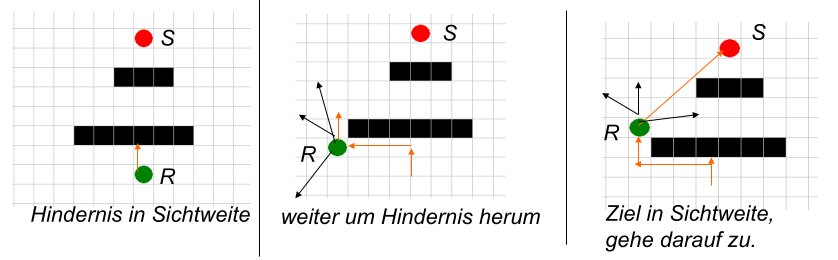
\includegraphics[width=\textwidth]{figures/kap3/bug-algo-1.png}
    \caption{Beispiel von Bug-Algorithmus Verfahren}
    \label{fig:bug-algo}
\end{figure}

\subsection{Problem mit dem Bug-Algorithmus}

In bestimmten Situationen (z.B siehe Abb. \ref{fig:bug-algo-prob}) ist der Roboter mit dem Ansatz in Abschnitt~\ref{bug-algo-1} nicht in der Lage, das Ziel zu finden.

\begin{figure}[H]
    \centering
    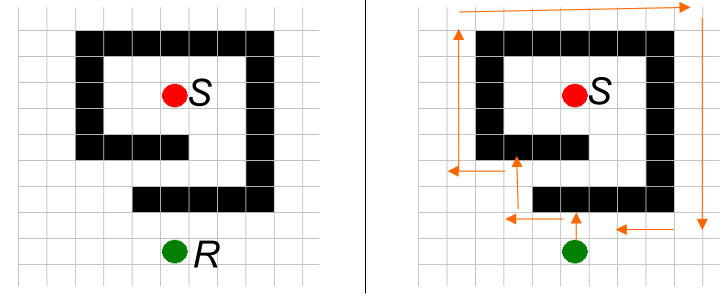
\includegraphics[width=0.8\textwidth]{figures/kap3/bug-algo-1-problem.png}
    \caption{Der Roboter kann das Ziel nicht sehen}
    \label{fig:bug-algo-prob}
\end{figure}

Der Algorithmus muss verbessert werden, z. B. durch Bewegen gegen den Uhrzeigersinn, um eine Bewegung in einem kontinuierlichen Kreis zu vermeiden.

\begin{figure}[H]
    \centering
    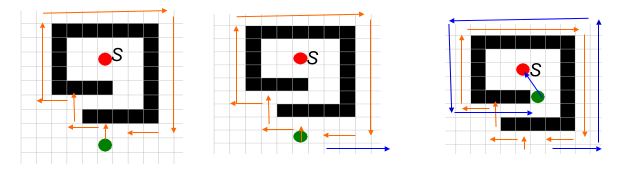
\includegraphics[width=\textwidth]{figures/kap3/bug-algo-1-fix.png}
    \caption{Gegen den Uhrzeigersinn bewegen, um das Ziel zu erreichen}
    \label{fig:bug-algo-fix}
\end{figure}